%! TEX root = main.tex

We first examined the performance of AmgXWrapper.
Figure \ref{fig:amgxwrapper-cons-1M} and \ref{fig:amgxwrapper-cons-15M} show the run time of solving Possion problems.
The former solves a smaller problem with $1$ million unknowns, and the latter has $15$ millions unknowns.
In each figure, on the left we have the performance before applying the consolidation mechanism in AmgXWrapper.
And on the right we show how the consolidation helps the performance.
The tests were done with NVIDIA V100 GPUs.

\begin{figure}[H]%
    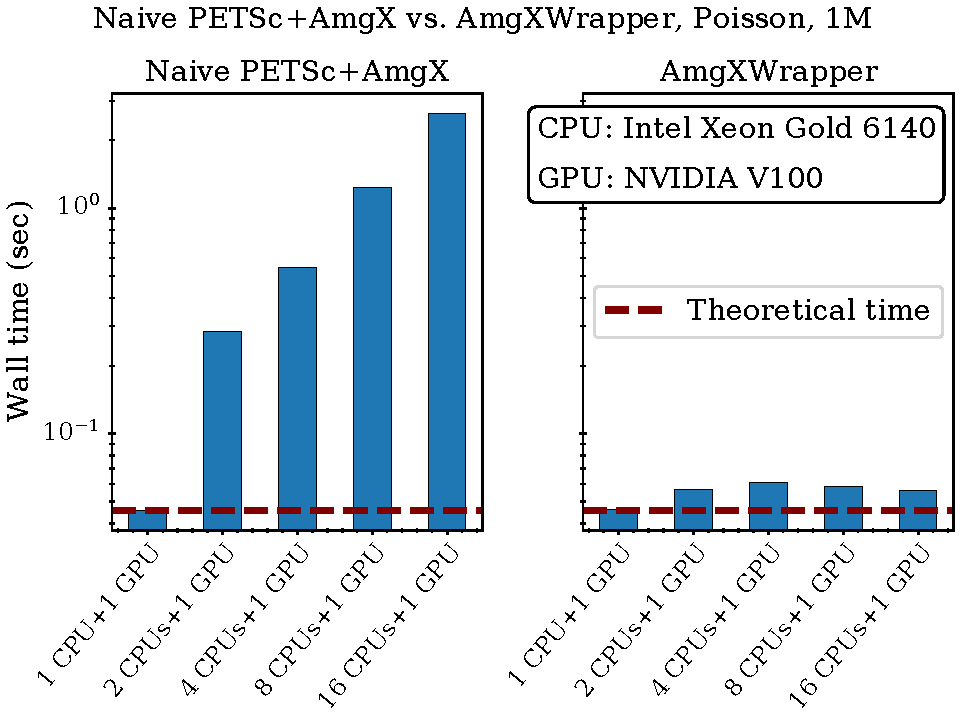
\includegraphics[width=0.6\linewidth]{amgxwrapper-consolidation-tests-poisson-1M}%
    \caption{AmgXWrapper benchmark: 3D Poisson problem w/ 1M unknowns and using 1 V100 GPU.}\label{fig:amgxwrapper-cons-1M}%
\end{figure}

\begin{figure}[H]%
    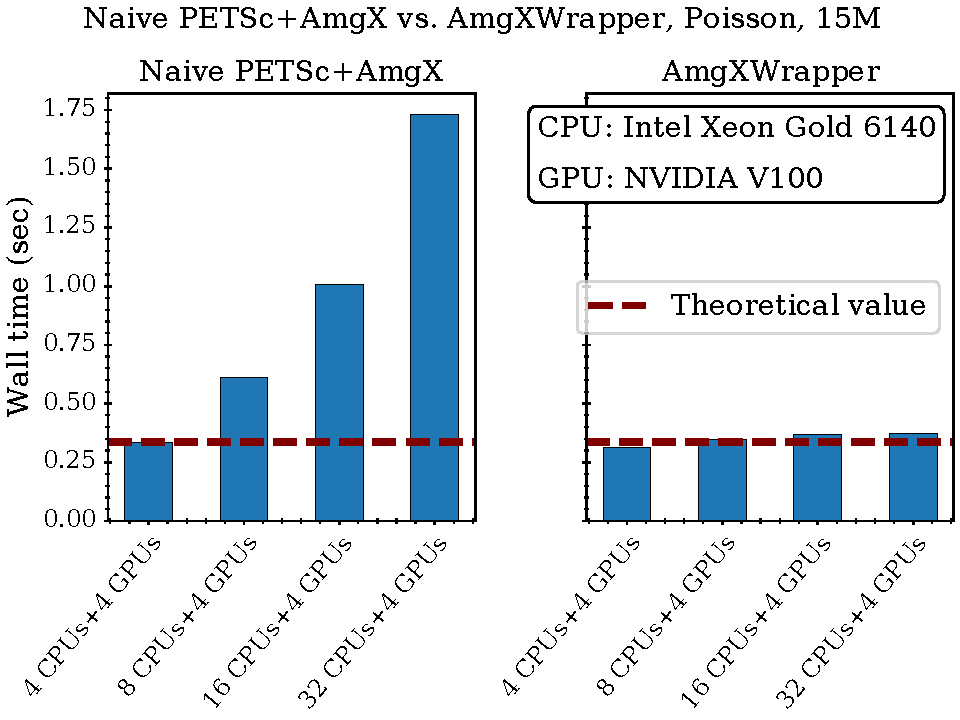
\includegraphics[width=0.6\linewidth]{amgxwrapper-consolidation-tests-poisson-15M}%
    \caption{AmgXWrapper benchmark: 3D Poisson problem w/ 15M unknowns and using 4 V100 GPUs.}\label{fig:amgxwrapper-cons-15M}%
\end{figure}

Bars in the figures represent the results of using different numbers of CPUs plus a fixed number of GPUs.
The smaller Poisson problem was solved with one GPU, while the larger problem was solved with 4 GPUs.
Using more CPUs speeds up the pre-processing stage, such as matrix creation because it means more subdomains and fewer unknowns per subdomain.
However, the run times of the solving stage should not be affected by the number of CPUs because the solver resides on GPUs completely, and we have a fixed number of GPUs.

Results in \ref{fig:amgxwrapper-cons-1M} and \ref{fig:amgxwrapper-cons-15M} show that this statement is not true for the plots on the left, that is, without consolidation. 
As more CPUs are used, run times grows linearly.
V100 was still the mainstream GPUs used on HPC clusters at the time of writing.
Yet the results show it was not designed for handling multiple tasks and does not handle well with resource competition.

The consolidation in the translation layer helps resolve the issue.
This mechanism consolidate and rearrange subdomains' matrices.
Rearranging is necessary as the performances of multigrid preconditioners may rely on the structures of submatrices on each GPU.
Plots on the right show that run times were close to a constant time regardless of how many CPUs were used.

The time used for consolidation was included in the solving stage shown in these two figures.
The smaller Poisson problem shows an overhead due to the consolidation.
However, for the larger problem, the overhead was not obvious as consolidation is a relative cheap operation compared to the actual solving. 

Next, in figure \ref{fig:amgxwrapper-speedups-15M} and \ref{fig:amgxwrapper-speedups-33M}, we show the speedups of GPU solvers versus CPU solvers on Poisson problems.
The former has $15$ millions of unknowns, while the latter has $33$ millions.
The plots also contains a visualization of the strong scaling.
The CPU tests used the conjugate-gradient (CG) solver from PETSc with the BoomerAMG preconditioner from Hypre.
The GPU tests used the CG solver and the classical multigrid preconditioner from AmgX.
Theoretically, these two configurations are comparable because AmgX's classical multigrid preconditioner was a re-implementation on GPU of BoomerAMG. 

\begin{figure}[H]
    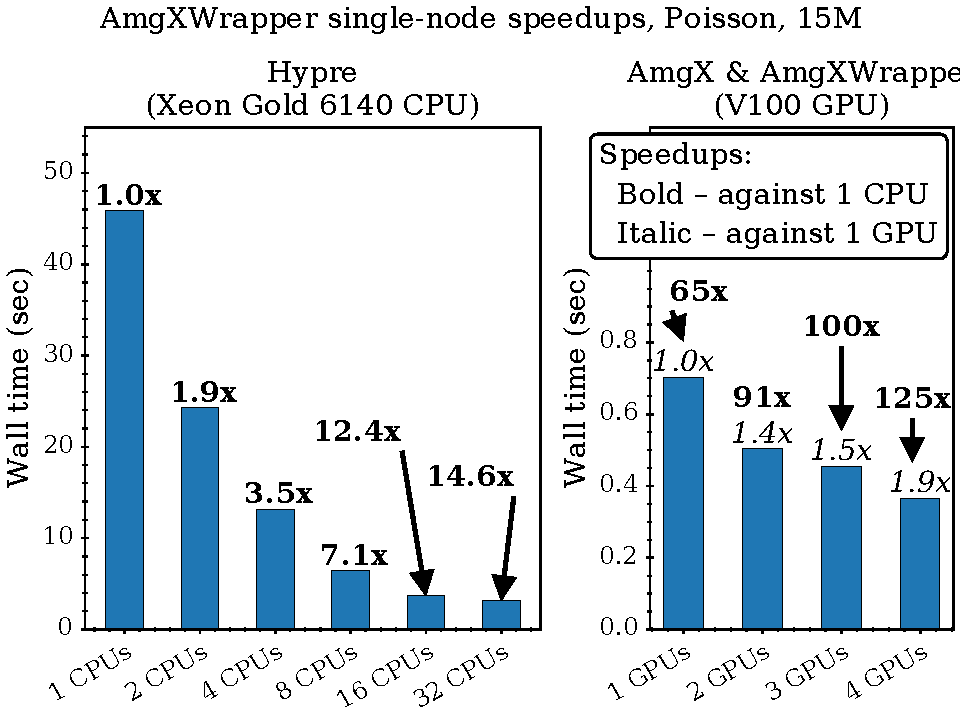
\includegraphics[width=0.6\linewidth]{amgxwrapper-proc-speedups-poisson-15M}
    \caption{Speedups of AmgXWrapper vs.\@ Hypre w/ 15M unknowns.}
    \label{fig:amgxwrapper-speedups-15M}
\end{figure}

\begin{figure}[H]
    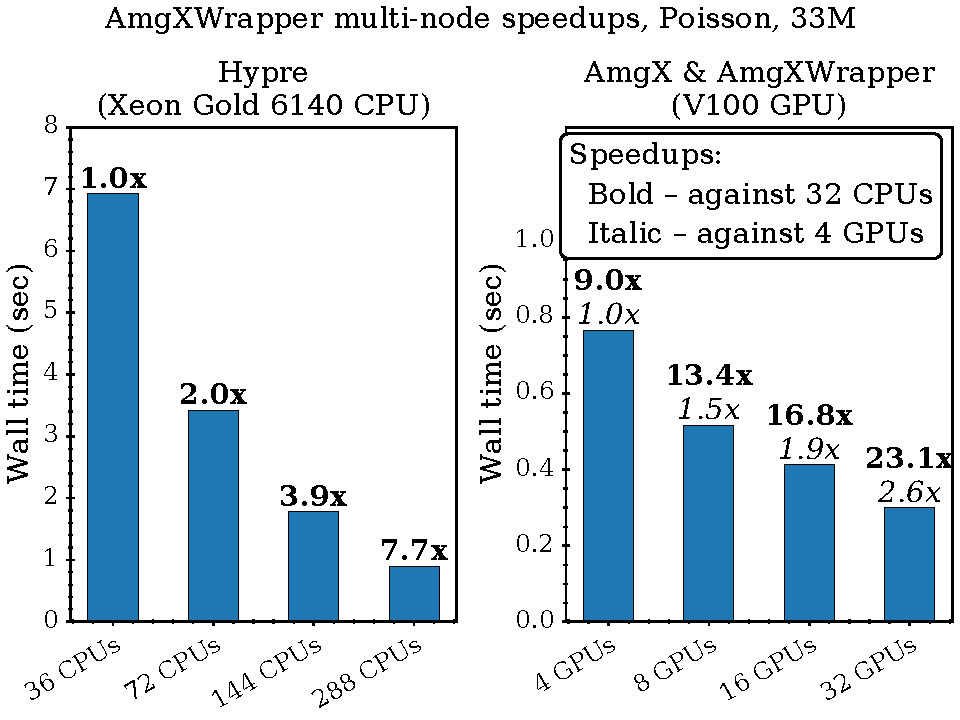
\includegraphics[width=0.6\linewidth]{amgxwrapper-node-speedups-poisson-33M}
    \caption{Speedups of AmgXWrapper vs.\@ Hypre w/ 33M unknowns.}
    \label{fig:amgxwrapper-speedups-33M}
\end{figure}

From the results, we observed a $65x$ speedup comparing 1 GPU to 1 CPU in the $15$-million problem and a $9x$ speedup comparing 4 GPUs to 36 CPUs in the $33$-million problem.
As a reference, at the time of writing, 4 V100 GPUs cost about $12$ thousand US dollars.
On the other hand, $36$ cores of CPUs consists of $2$ Xeon Gold 6140 chips, which cost around $2$ thousand US dollars\footnote{Xeon Gold 6140 was descontinued at the time or writing. The price we show here was the market value at the time, while the official suggested price for $2$ brand-new chips was around $4,800$ US dollars.}.
If we naively compare the results base on the monetary cost of the GPUs and CPUs, we would observe a speedup of about $1.5x$ (4 V100 GPUs versus 218 CPU cores).
However, as CPUs and GPUs work under different hardware configurations and setups, this monetary-based comparison is not fair in the real world.
For example, $6$ CPU chips may require $3$ complete computing nodes and an HPC cluster, while 4 V100 GPU can completely reside in one single workstation or even a personal desktop.
Under this argument, both the hardware cost and human labor cost (for maintenance) of CPUs will be much higher, and the speedups and cost saving from GPUs will be much more attractive.
Unfortunately, we were not able to get the cost estimation of a $3$-node HPC cluster and hence were not able to continue on the monetary cost comparisons.
Nevertheless, we hope our arguments can provide an impression on the hardware costs as these costs are often ignored in literature of performance benchmarks.

In terms of strong scaling, CPU solvers tended to show a better strong scaling.
For example, if we translate the speedup in the CPU results to strong scaling efficiencies for the smaller problem were about 95\%, 88\%, 88\%, 78\%, and 46\%, respectively.
And those of the larger problem were 100\%, 98\%, and 96\%.
In the GPU results, the strong scaling efficiencies of the small problem were 70\%, 50\%, and 48\%, while those of the larger problem were 75\%, 47\%, and 32\%.
From this viewpoint, CPU solvers give a better predictability on required resources and time-to-solutions. 

Finally, we were interested the actual performance gain in real flow simulation.
Figure \ref{fig:petibm-speedups-15M-small} and \ref{fig:petibm-speedups-15M-large} show the high-level performance profiling of PetIBM using a 3D flying-snake simulation \cite{krishnan_lift_2014,krishnan_cuibm_2017}.
The number of cells is $15$ millions, meaning there were about $45$ millions unknown in the velocity system and $15$ million unknowns in the pressure system.
The snake was discretized to $2,925$ Lagrangian points, meaning the forcing system has $8,775$ unknowns.

\begin{figure}[H]
    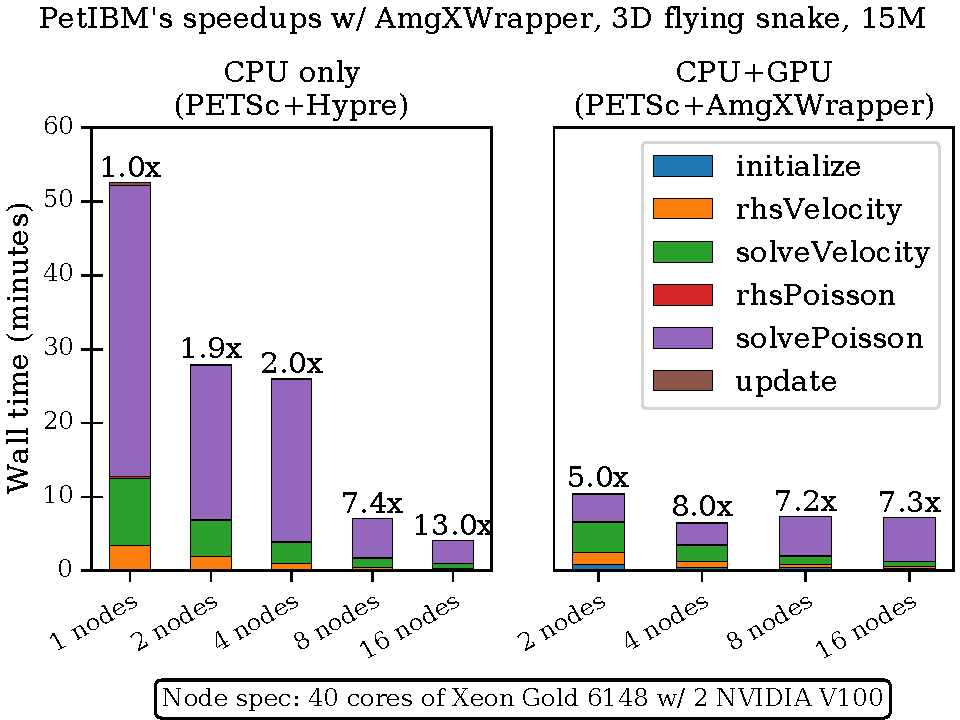
\includegraphics[width=0.6\linewidth]{petibm-speedups-scaling-small-gpu}
    \caption{Speedups of PetIBM: 2 V100 per node}
    \label{fig:petibm-speedups-15M-small}
\end{figure}

\begin{figure}[H]
    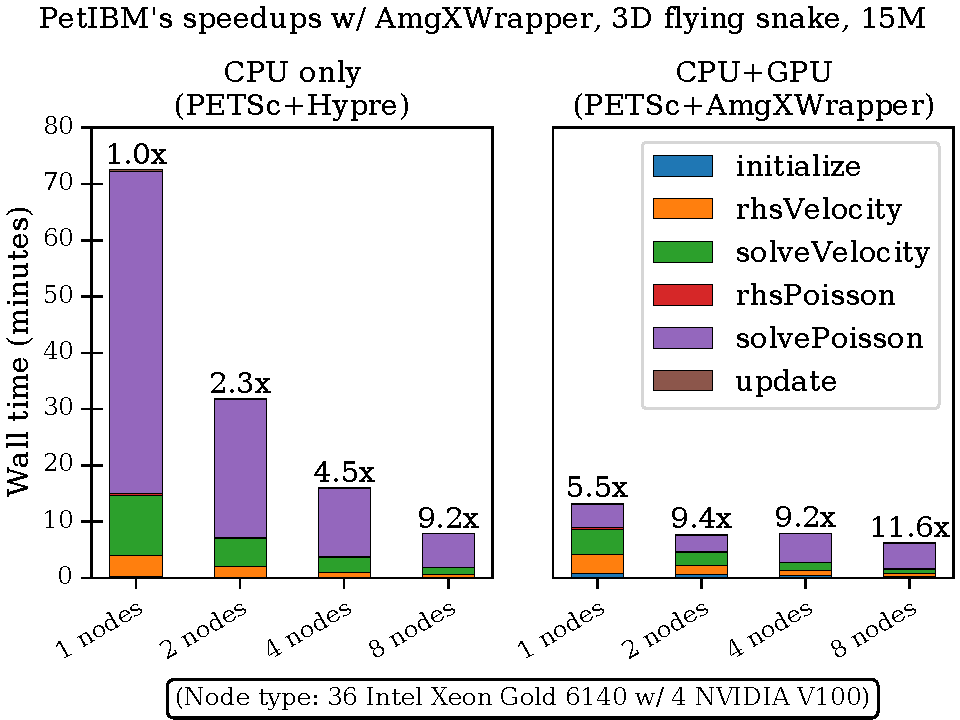
\includegraphics[width=0.6\linewidth]{petibm-speedups-scaling-large-gpu}
    \caption{Speedups of PetIBM: 4 V100 per node}
    \label{fig:petibm-speedups-15M-large}
\end{figure}

In CPU-only simulations, PetIBM solved velocity systems with the GAMG preconditioner and pressure systems with BoomerAMG preconditioner.
In CPU-GPU mixed simulations, the preconditioners for velocity and pressure systems are block-Jacobi and classical multigrid from AmgX, respectively.
The underlying Krylov solvers are the bi-conjugate gradient stabilized solver from either PETSc or AmgX.
The forcing systems in both types of simulations were solving by LU decomposition using distributed SuperLU.
This is the only part solved on CPU for the CPU-GPU mixed simulations.

The two figures show the performance speedups comparing pure-CPU and CPU-GPU-mixed simulations on two different clusters: one with 2 V100 per node, while the other one with 4 V100 per node.
We conducted the simulations on two different to ensure the results has generalizability.
The results from both clusters agree with each other.
We observed that one 4-GPU node or two 2-GPU nodes are equivalent roughly to 5 pure-CPU nodes.
The difference between the two clusters lies in that the 4-GPU nodes had less internode communication and hence had better performance and scalability.
% vim:ft=tex